\documentclass[aip,pop,amsmath,amssymb,reprint,superscriptaddress]{revtex4-1} %preprint version
\usepackage{graphicx}% Include figure files
\usepackage{dcolumn}% Align table columns on decimal point
\usepackage{bm}% bold math

    \renewcommand{\topfraction}{0.9}    % max fraction of floats at top
    \renewcommand{\bottomfraction}{0.8}    % max fraction of floats at bottom
    \setcounter{topnumber}{2}
    \setcounter{bottomnumber}{2}
    \setcounter{totalnumber}{4}     % 2 may work better
    \setcounter{dbltopnumber}{2}    % for 2-column pages
    \renewcommand{\dbltopfraction}{0.9}    % fit big float above 2-col. text
    \renewcommand{\textfraction}{0.07}    % allow minimal text w. figs
    \renewcommand{\floatpagefraction}{0.7}    % require fuller float pages
    \renewcommand{\dblfloatpagefraction}{0.7}    % require fuller float pages
    \setlength{\abovecaptionskip}{5pt}
    \setlength{\belowcaptionskip}{5pt}
    \setlength{\parskip}{0pt}
    \setlength{\textfloatsep}{5pt} 

\begin{document}
\title{Signatures of dissipation in an MHD turbulent experiment}
\author{D.A. Schaffner}
\affiliation{Department of Physics, Bryn Mawr College}
\author{A. Rock}
\author{M.R. Brown}
\affiliation{Department of Physics and Astronomy, Swarthmore College}
\date{\today}
\begin{abstract}
The instabilities observed on the Large Plasma Device (LAPD) [W. Gekelman, \textit{et. al}, Rev. Sci. Instr. \textbf{62}, 2875 (1991)] are explored in conjunction with a the ability to finely adjust azimuthal flow and flow shear.

\end{abstract}
\maketitle

\section{Introduction}

Turbulent dissipation is an important topic in astrophysical plasmas. It involves questions including the solar corona heating problem and the radial temperature of the heliosphere. Despite decades of in-situ observation of the solar wind, the exact process of how large scale kinetic and magnetic energy ejected from the sun into the heliosphere gets transferred to the thermal motions of the plasma constituents. For highly collisional magnetic turbulence (or liquid metal turbulence), resistivity of the plasma typically fulfills the dissipation role as currents in the plasma deposit energy to particles through collisions. However, in extremely sparse, hot and nearly collisionless plasmas such as the solar wind, resistivity cannot play such a role. The alternative mechanisms typically fall into two main groups: coupling between wave fluctuations and particle motion (including Landau damping or cyclotron resonance) or though the formation of current sheets and reconnection layers which convert magnetic energy into kinetic flows, which can in turn be thermalized.

In parallel with continued in-situ exploration of these phenomena, production and analysis of magnetized turbulent plasma in the laboratory can be an extremely useful for helping to understand what processes are possible in such a plasma and to what extent these various types of dissipation mechanisms are present or contribute to turbulent dissipation. While measurement of turbulent parameters in a laboratory plasma can have a variety of advantageous over in-situ satellite measurement (including higher spatial resolution and control of plasma parameter space), other diagnostic challenges do arise.  In this paper, we present a variety of analysis techniques aimed at identifying and characterizing turbulent dissipation signatures in a laboratory magnetic turbulent plasma—the plasma wind tunnel in the Swarthmore Spheromak Experiment (SSX). We present a basic outline of the techniques including advantageous and disadvantages of its use, as well as discuss possible interpretations of the results in the context of dissipation mechanisms. More importantly however, this paper attempts to synthesize the results of multiple techniques to make conclusions on the nature of turbulent dissipation in this plasma.

Since turbulence is being explored in a laboratory setting, some clarification of the specific type of turbulence being investigated needs to be made. Plasma turbulence in the literature typically refers to the relative large fluctuations of plasma parameters including density, temperature and floating potential, within the framework of a stiff background magnetic field. It is associated with the formation and relaxation of gradients (such as pressure gradients in edge plasmas or ion temperature gradients in fusion plasma cores). In such systems, energy can be injected or dissipated at multiple scales, sometimes both occurring at the same scale. In contrast, astrophysical plasmas exhibit turbulence that is more fluid-turbulence like. That is, there tends to be a very large separation of energy injection and dissipation scales (and typically no formation of large scale spatial gradients. Energy is injected at the largest scales of the system and energy dissipated at scales often many orders of magnitude smaller. This type of turbulence is often referred to as magnetohydrodynamic turbulence as opposed to the gradient-driven turbulence described above. Of course, unlike conventional fluid turbulence, plasma, the collective behavior and interaction of plasma parameters makes MHD turbulence a significantly more challenging system to understand. Nevertheless, the largest MHD turbulence systems known typically exhibit a similar type of Kolmogorov scaling of energy as observed in conventional fluid turbulence. 

The challenge in exploring this type of turbulence in the laboratory arises in how to faithfully reproduce the elements of MHD turbulence while avoiding formation of gradients. This requires avoiding typical laboratory plasma generation techniques including cathode sources and background fields. As will be described below, MHD turbulence is generated in SSX using plasma gun sources and flux-conserving boundaries which allow for the injection of turbulent magnetized plasma which can evolve dynamically without a background field. While plasma generated in this way cannot completely reproduce the conditions observed in heliosphereic plasmas, it represents a closer approximation than other laboratory devices have been able to make.

\section{Combining Signatures of Turbulent Dissipation}

Since the model of scale-separated turbulence is best represented by an energy spectrum as a function of scale, the standard analysis tool is spectral analysis of magnetic fluctuations. Ideally, fields could be measured spatially in order to decompose fluctuations into wavenumber space; however, most measurements are made at a single location, so temporal fluctuation spectra are used as a proxy, though turbulence theories generally do not make predictions for the behavior of such time spectra. If the turbulent system moves past the measurement point at a rate faster than the temporal change in the system, a direct corresponsdance between temporal and spatial spectra---called the Taylor Hypothesis. This procedure is done in the solar wind, for example, for measurements made in the at 1AU or beyond where solar wind velocities far exceed the temporal evolution scales. Such approximations cannot be as definitively made in this laboratory experiment; thus, spectra are presented as functions of measurement frequency rather than scale.

At any rate, the typical signature of turbulent dissipation extracted from either spatial or temporal spectra is a steepening of the spectrum at decreasing scale or increasing frequency just beyond the inertial range, which is itself characterized by Kolmogorov scaling (a functional form of $k^{-5/3}$ or $f^{-5/3}$). This transition indicates an energy sink in the process. While within the inertial range, magnetic energy cascades from larger to smaller scales, but remains magnetic energy, beyond the inertial range, this magnetic energy becomes converted into other forms. In pure Kolmogorov theory, this energy becomes thermalized, but more complicated plasma systems, the energy could conceivable be transferred into particle flows, coherent modes, or radiation in addition to heat. These added complexities make interpretation of dissipation mechanisms with spectra alone potentially difficult. 

Ultimately, the goal for these analyzes is to determine the physical nature of the mechanism of the dissipation. While a steepening spectrum indicates the possibility of some type of dissipative mechanism occurring, it cannot immediately indicate the type of mechanism in question. The technique does provide some quantitative information. The location of the onset of steepening in wavenumber or frequency space can indicate the possible scale at which the mechanism operates (or begins to operate). In the solar wind, a steepening away from Kolmogorov scaling is seen to occur near scales associated with both the ion gyroraduius and the ion inertial length. The scaling of the dissipation range can be informative, as well. For example, a observed scaling of $f^-7/3$ in the dissipation range could be indicative of the presence of a particular mode activity associated with the dissipation. It is here where comparison to the other analysis techniques can be illuminating. In particular, the intermittent character of the plasma can be exampled using probability distribution functions of increments and structure functions. Observation of such intermittency can be indicative of the formation of current sheets or reconeection layers in the turbulent plasma which in turn hints at the mechanism converting magnetic energy into particle flows. Higher order structure function analysis can also be used to unearth the fractal scaling nature of the plasma. A relatively new technique called permutation entropy and statistical complexity can also be used to explore a distinction between a chaotic versus a stochatisic process. For instance, an increase in complexity might be associated with the non-linear interaction of linear modes.

The remainder of this paper focuses on the application of the various analysis techniques described using a laboratory MHD turbulent plasma as a case study.

\section{Experimental Description}

The results presented in this paper are from measurements made in the extended MHD wind-tunnel configuration of the Swarthmore Spheromak Experiment. This mode of operation consists of a coaxial plasma gun source at one end of a $2.5$m long, $15.5$cm diameter copper cylinder, as indicated in Figure~\ref{fig:diagram}. The operation of the gun source has been described in previous work. For these results, the gun was operated with a stuffing flux of $1.3$mWb, and a discharge voltage of 4kV. The resulting plasma plume travels approximately $40$km/s as measured by the time-of-flight of magnetic structures. Measurements of magnetic field fluctuations are measured using magnetic pick-up coils or B-dot probes. The data presented here is from a single location, $24$cm from the end of the gun source electrode, as indicated in the Figure. Plasma gun discharges last on the order of $120\mu$s, but the analysis window for this data was restricted to $28$ to $58\mu$s, where fluctuations are fairly stationary. Fifty shots are uses to generate an ensemble average for each analysis technique utilized.

\begin{figure*}
\centerline{
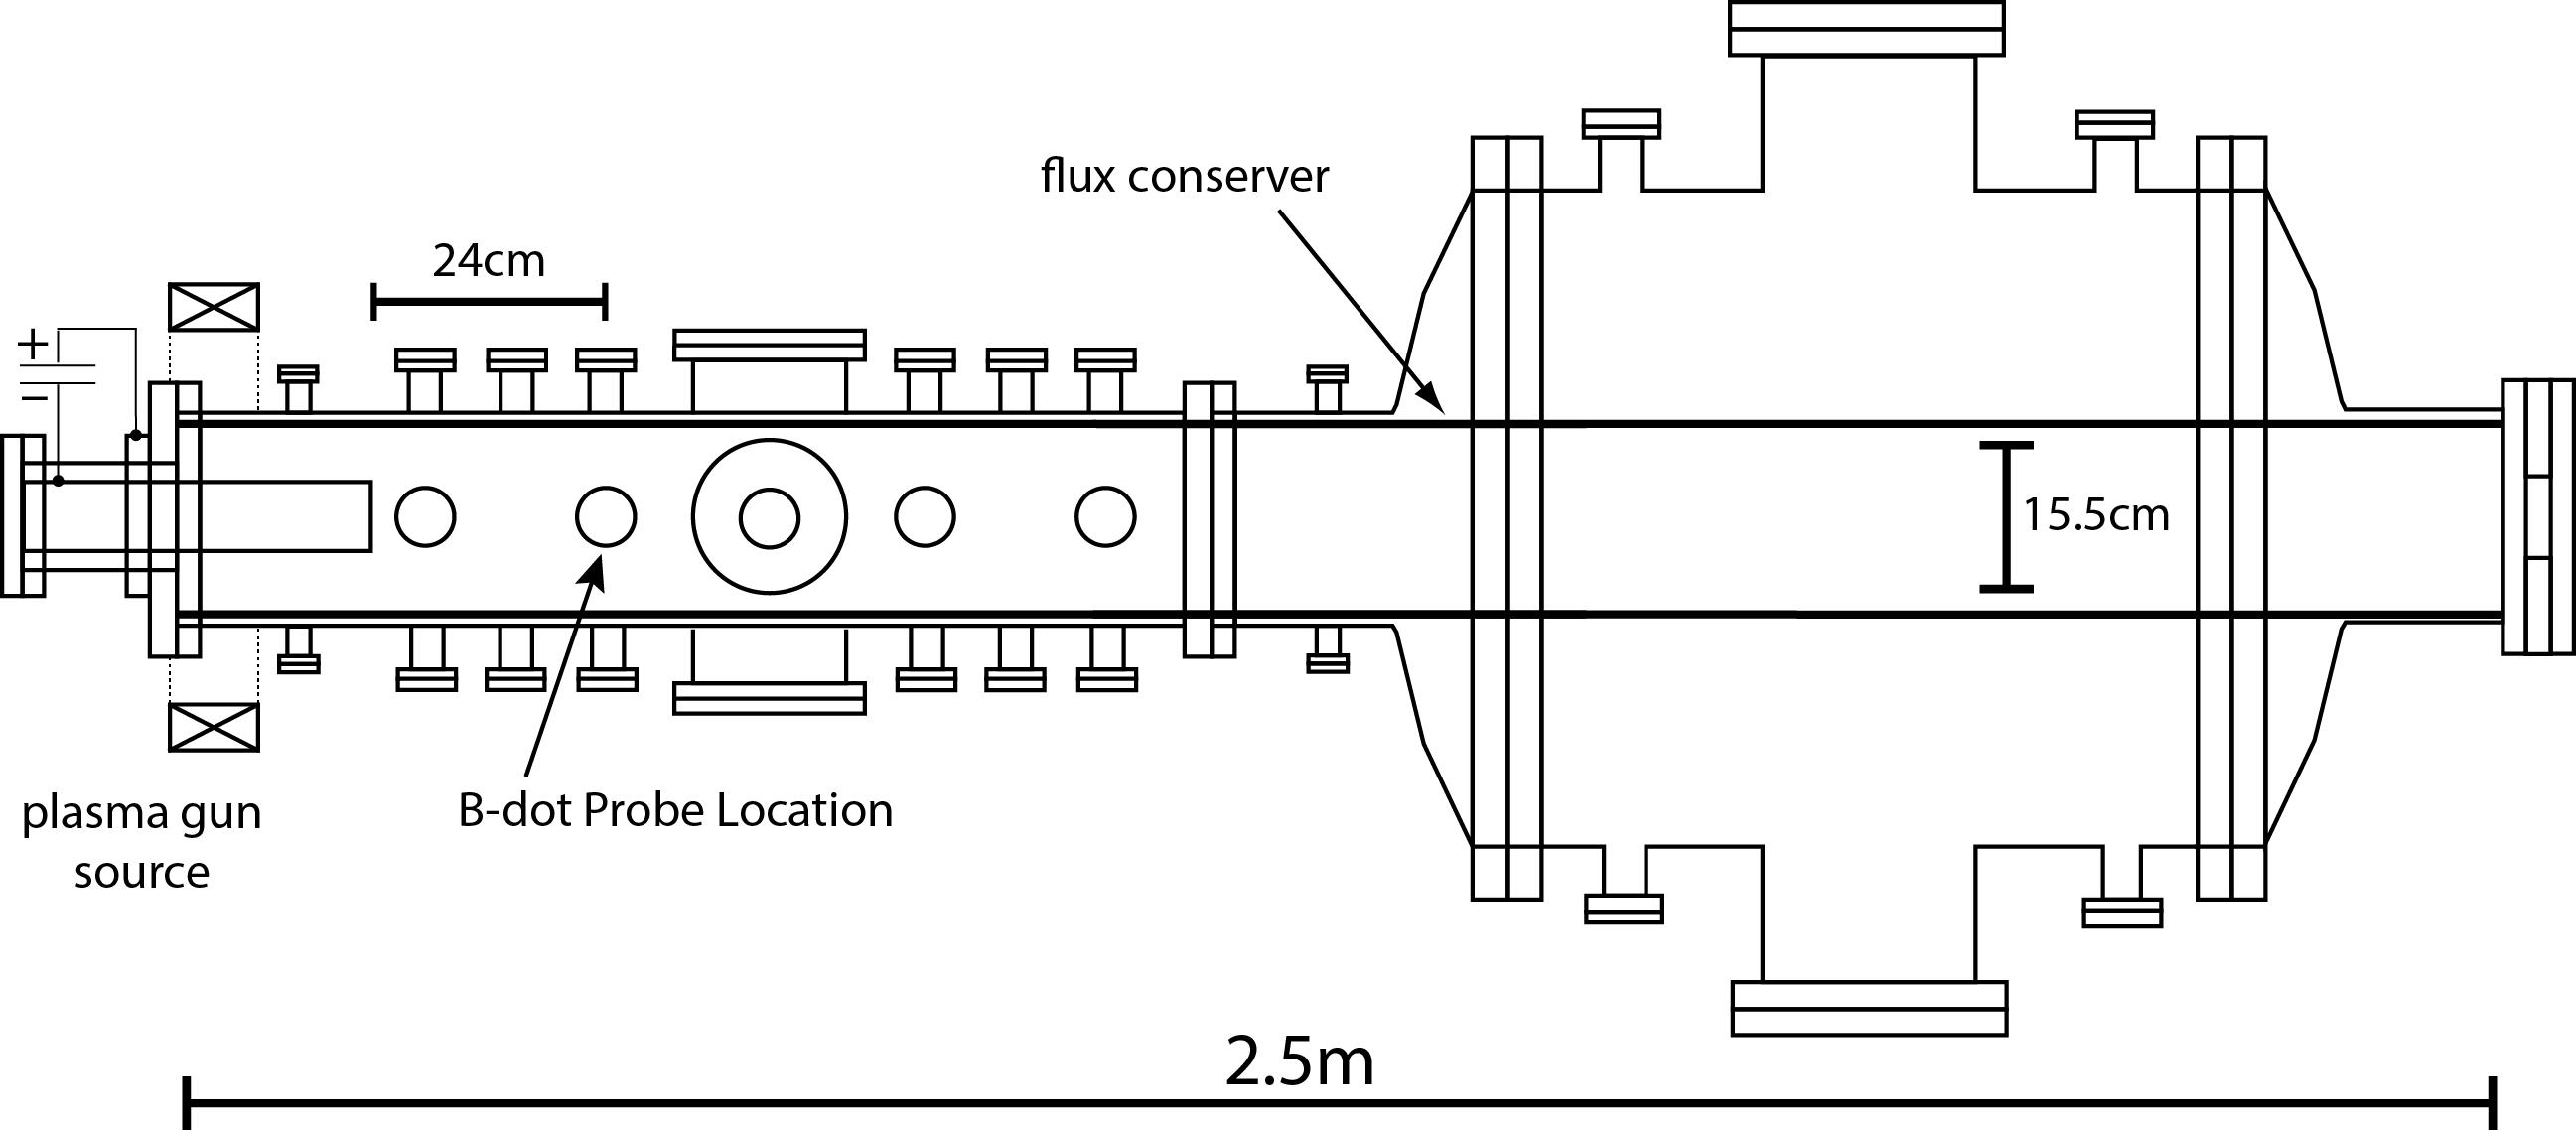
\includegraphics[width=17cm]{tunnel_2p5m_TurbDissDPPpaper.png}}
\caption{\label{fig:diagram}}
\end{figure*}

\section{Results}

\begin{figure}
\centerline{
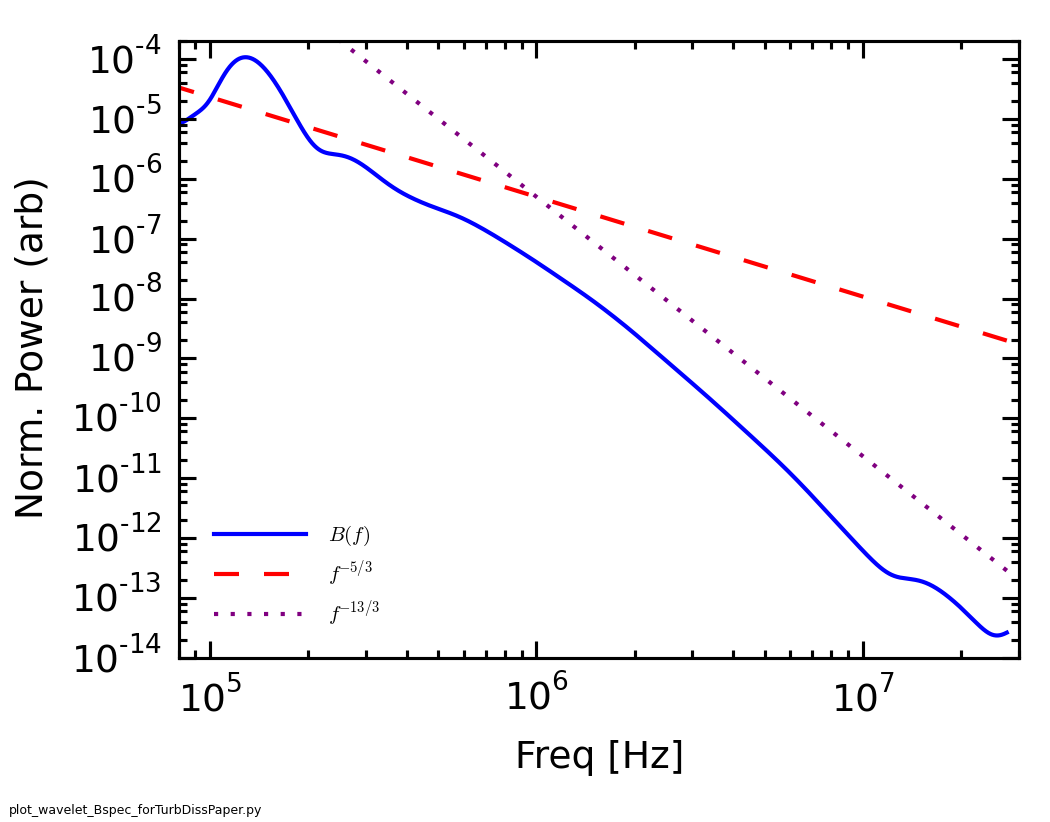
\includegraphics[width=8.5cm]{Young_spectra.png}}
\caption{\label{}}
\end{figure}

\begin{figure}
\centerline{
\includegraphics[width=8.5cm]{PE_SC_flatness.png}}
\caption{\label{}}
\end{figure}

\section{Conclusions}


\providecommand{\noopsort}[1]{}\providecommand{\singleletter}[1]{#1}%
\begin{thebibliography}{10}

\bibitem{schaffner12}
D.A. Schaffner, T.A. Carter, G.D. Rossi, D.S. Guice, J.E. Maggs, S.Vincena and B. Friedman, Phys. Rev. Lett. {\bf 109}, 135002 (2012).


\end{thebibliography}
\end{document}
